\documentclass[../main/main.tex]{subfiles}

\begin{document}

Figure \ref{profile_vs_multiplication_xmueout_iso} shows the profile when the scattering angle is allowed to lie in the interval $\mu_{\text{out}} \in [-1,1]$. Figure \ref{profile_vs_multiplication_xmueout_pos} shows the same computations, but with $\mu_{\text{out}} \in [0, 1]$

\begin{figure}[!htp]
\centering
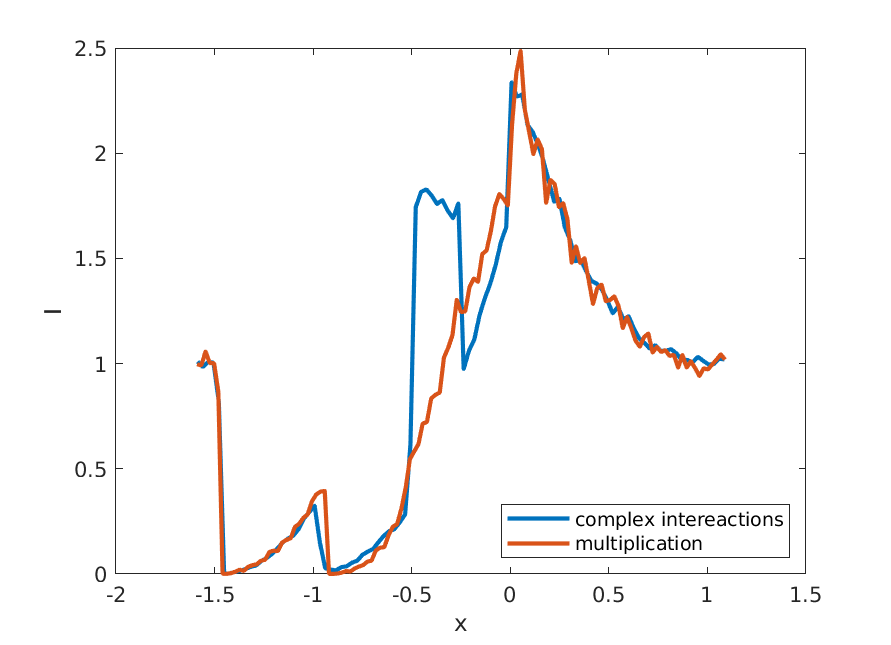
\includegraphics[width=0.7\textwidth]{../../two_resonance_lines/figures/multiplication_vs_complex_interactions_xmueout_iso.png}
\caption{Comparison with multiplied profile ($\mu_{\text{out}} \in [-1, 1]$)}
\label{profile_vs_multiplication_xmueout_iso}
\end{figure}

\begin{figure}[!htp]
\centering
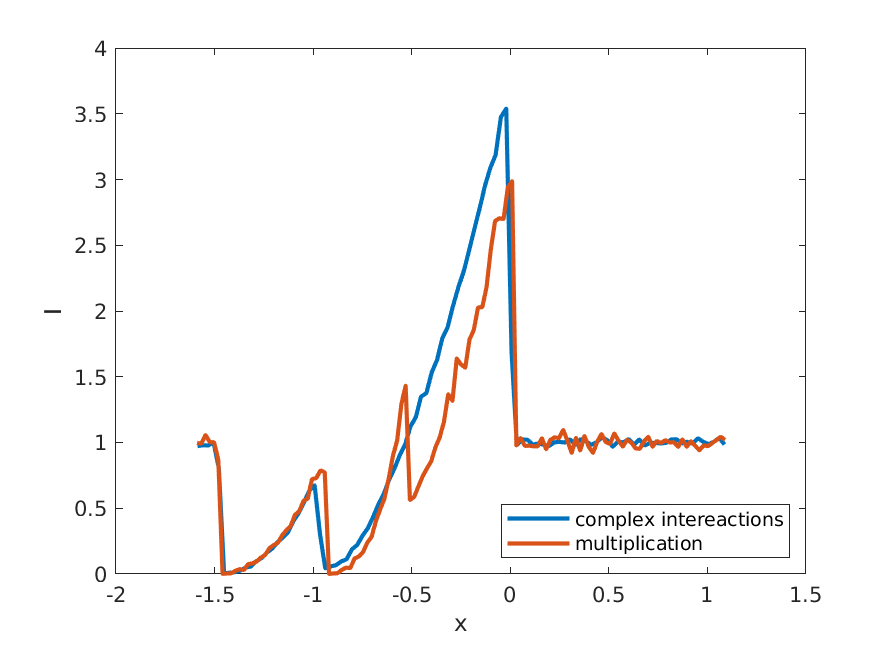
\includegraphics[width=0.7\textwidth]{../../two_resonance_lines/figures/multiplication_vs_complex_interactions_xmueout_pos.png}
\caption{Comparison with multiplied profile ($\mu_{\text{out}} \in [0,1]$)}
\label{profile_vs_multiplication_xmueout_pos}
\end{figure}

Loosely speaking, one can understand this result because in Figure \ref{profile_vs_multiplication_xmueout_pos}, photons are not allowed to be backscattered to the first resonance line.


\end{document}